\documentclass{article}%
\usepackage[T1]{fontenc}%
\usepackage[utf8]{inputenc}%
\usepackage{lmodern}%
\usepackage{textcomp}%
\usepackage{lastpage}%
\usepackage{authblk}%
\usepackage{graphicx}%
%
\title{Elevated Maspin Expression Is Associated with Better Overall Survival in Esophageal Squamous Cell Carcinoma (ESCC)}%
\author{Eric Mason}%
\affil{Department of Pediatrics and Molecular and Cellular Oncology, The University of Texas M. D. Anderson Cancer Center, Houston, TX, USA}%
\date{01{-}01{-}2013}%
%
\begin{document}%
\normalsize%
\maketitle%
\section{Abstract}%
\label{sec:Abstract}%
San Diego women with an aggressive form of ovarian cancer that results in changes to their physical appearance are up to 87 percent more likely to develop the disease if their tumors are found and studied with the ability to improve their outcome through targeted treatment.\newline%
Researchers have conducted research that could improve the likelihood of these women to live longer lives.\newline%
Screening and personalized therapy is the next frontier in developing ovarian cancer treatments. But treatment does not eradicate the cancer, so maintaining a healthy lifestyle may still need to be a part of the solution.\newline%
Researchers discovered by studying a woman with an especially aggressive type of ovarian cancer who undergoes a series of tests to determine whether she has a malignant genetic mutation, an abnormal gene signature or an immune suppressor gene.\newline%
Prognostic test results confirmed that the patient did not have normal cell differentiation and survival in the gene carriers was actually low. This was the first way a biomarker found in ovarian cancer cells was confirmed in an animal model.\newline%
The ovarian cancer types with abnormal development include Waldenstroms disease, Gynecomastia subtype 2/4A, BRCA{-}1 and BRCA{-}2. This type of cancer is relatively uncommon in women, estimated to occur in less than 4,000 women annually.

%
\subsection{Image Analysis}%
\label{subsec:ImageAnalysis}%


\begin{figure}[h!]%
\centering%
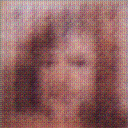
\includegraphics[width=150px]{500_fake_images/samples_5_397.png}%
\caption{A Man Is Standing In Front Of A Mirror}%
\end{figure}

%
\end{document}